\chapter[Applications of the Conservation Laws]{Applications of the 
Relativistic Conservation Laws}
\label{chapter:relativity_app}

%\section*{Objectives}
%\begin{objectives}
%\item Describe increases and decreases in mass associated with processes
%that release or absorb kinetic energy.
%\item Apply the relativistic conservation laws to ``explosions,'' in
%which one particle decays into two particles, including cases in
%which one or both outgoing particles have zero rest mass.  
%\item Do the same for simple collisions with all particles traveling
%along a line.
%\item Be able to describe the processes of nuclear fusion and fission,
%and explain how these processes result in kinetic energy production.  
%\item Given information about nuclear masses, calculate the amount of
%kinetic energy gained in a fusion or fission process.
%\end{objectives}

\section{Introduction}

You should now understand why Einstein's postulates
require new definitions of momentum and energy.  The classical
momentum is not conserved, nor in general is the total mass of the
particles in an interaction.  In place of these, relativistic momentum
and relativistic energy are conserved, and they are conserved in any
inertial frame.  

In this chapter, we apply these new, relativistic conservation laws to 
analyze collisions and decays of subatomic
particles.  The key result in these applications is the ability for
matter to be converted into kinetic energy and vice-versa.  In relativistic
collisions, the amount of matter that you start with is not the same
as the amount of matter that you finish with!  We also discuss the
principles behind nuclear fission and nuclear fusion.

\section{Changes of Rest Energy}
  Much of the light you see comes from changes in rest energy of
atoms.  Examples are sunlight, light from a candle flame, a lightning
flash, light emitted by a fluorescent lamp, light from the phosphor
coating on the screen of a television set or a video monitor, and
laser light.  In all these examples, the basic mechanism is that an
atom in an ``excited'' state releases its energy in the form of a
photon, with the atom going into its ground (lowest possible) state,
or into an excited state of lower energy.  We can represent the
emission process by the simple reaction equation

\begin{equation}
{\bf A}^\ast \rightarrow {\bf A} + \gamma. 
\label{eq:photon_emission}
\end{equation}
Here ${\bf A}^\ast$ represents the excited atom, ${\bf A}$ the atom in its
ground or lowest state, and $\gamma$ (Greek {\em gamma}) the photon.

\begin{figure}[tbp]
\begin{center}
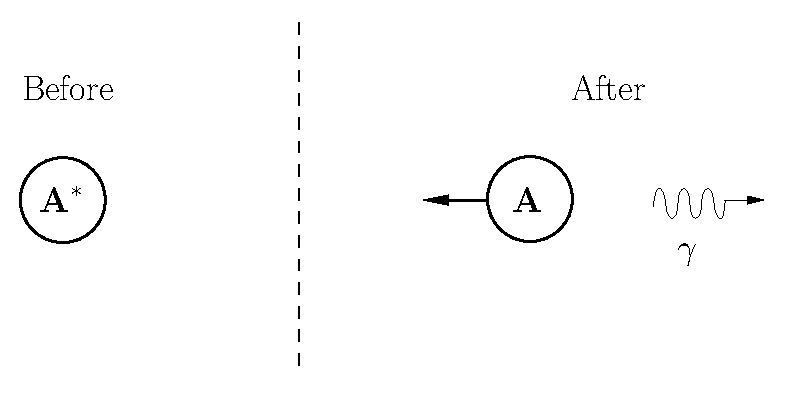
\includegraphics[width=3.5in]{relativity_conservation/photon_emission1.eps}
\end{center}
\caption{An excited atom emits a photon and recoils.}
\label{fig:photon_emission1}
\end{figure}

In Fig.~\ref{fig:photon_emission1}, the excited atom is shown at rest,
so all of its energy is rest energy and it has no momentum.  But the
photon has energy, and from the relation $E = pc$, it also has
momentum.  And because momentum must be conserved, the atom recoils.
We can write the conservation of energy equation for the reaction in
Eq.~(\ref{eq:photon_emission}) as follows
\begin{equation}
\text{Rest Energy of ${\bf A}^\ast$} = \text{Energy of ${\bf A}$} 
+ \text{Energy of photon}.
\end{equation}
     
Because both the kinetic energy of ${\bf A}$ and the photon energy are
positive numbers, the rest energy (i.e., the mass) of the
excited-state atom must be greater than that of the ground-state atom.
Therefore, in the emission process rest energy, i.e., mass, is
converted to kinetic energy.
     
When light is absorbed by an atom, exactly the opposite effect occurs.
The atom begins in its ground state, absorbs the photon energy and
goes into an excited state.  Again, by conservation of energy, the
excited atom must have more rest energy than the ground-state atom.

Another everyday example of changing rest energy occurs in chemical
reactions.  For example, the reaction for the oxidation of a carbon
atom
\begin{equation}
\text{C} + \text{O}_2 \rightarrow \text{CO}_2
\end{equation}
is known to release energy in the form of one or more photons.
Therefore the sum of the masses of C and O$_2$ must be greater than
the mass of the carbon dioxide molecule.  The change in rest energy in
the case of chemical reactions is typically on the order of
$1\units{eV}$ (or $1.6\times 10^{-19}\units{J}$).  Much larger
energies, on the order of $1\units{MeV}$, are involved in nuclear
reactions.  An example of a nuclear reaction is the decay of a neutron
into a proton, an electron, and an electron antineutrino:
\begin{equation}
n \rightarrow p + e^- + \bar{\nu}_e.
\end{equation}
Here the excess mass of the neutron over the mass of the proton plus
electron (the electron antineutrino has very small mass) is converted
to the kinetic energy of the three reaction products.

Another important example of changes in rest mass is the production of
new particles in a high energy particle accelerators.  In these
accelerators high-speed particles are shot at target particles and
some of the kinetic energy of the incoming particles is converted to
rest energy.  In this way hundreds of new particles, most with
lifetimes between $10^{-10}$ and $10^{-23}\units{s}$, have been
produced.  You'll learn more about these new particles next semester
in PHYS 212.

\section[General Strategy]{General Strategy for 
Applying the Relativistic Conservation Laws}


 In a typical problem you are given information about the particles
before an interaction and asked to compute certain properties of the
outgoing particles after the interaction.  You do this by writing down
equations that express the fact that the sum of the incoming momenta
is equal to the sum of the outgoing momenta and the sum of the
incoming energies is equal to the sum of the outgoing energies.  What
quantities should be used in writing these equations?  Here is some
time-saving advice.
\begin{quote}
Always write the conservation of momentum and conservation of energy
equations in terms of momentum and energy or mass variables, never in
terms of velocity or kinetic energy.
\end{quote}

This rule keeps the algebra as simple as possible --- it gets around
having to solve simultaneous equations with the $\sqrt{1-v^2/c^2}$
terms that can make the algebra messy.  For example, if you are given
the velocity of one or more particles in the problem statement, first
calculate the momentum and energy of each particle from the given
velocities.

A second piece of advice:
\begin{quote}
When working with ``eV'' units (e.g., MeV for energy, MeV/$c$ for
momentum, MeV/$c^2$ for mass), don't ever put any numbers in for the
speed of light $c$.  Just leave it as ~``$c$.''  The units will then
automatically take care of themselves.
\end{quote}

For example, if you have an motionless electron, its energy can be
obtained from $E^2 = p^2c^2+m^2c^4$. For a motionless electron  $p = 0$, 
so $E= mc^2 = 0.511\units{MeV/$c^2$}\times c^2 = 0.511\units{MeV}$.  
(See section \ref{section:rel-units}.)

\begin{example}{Emission of a photon by a nucleus.}
\label{ex:nuclear_decay}
An excited atomic
nucleus, of mass $5.00\units{GeV/$c^2$}$ and at rest, as in
Fig.~\ref{fig:photon_emission2}, decays to its ground state by
emitting a photon of energy $2.00\units{GeV}$.  Calculate the recoil
velocity and mass of the ground-state nucleus.
\solution
First draw a picture, and label each particle with its value of
energy and momentum.  Before the decay the excited nucleus has zero
momentum because it is at rest.  And from $E^2 = p^2c^2 + m^2c^4$, with 
$p =0$, we know its energy is the same as its rest energy, namely 
$5.00\units{GeV}$.

\begin{figure}[tbp]
\begin{center}
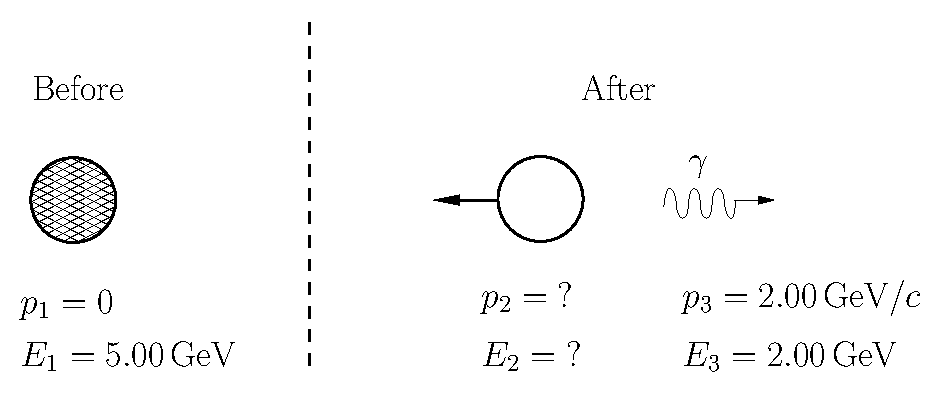
\includegraphics[width=4in]{relativity_conservation/photon_emission2.eps}
\end{center}
\caption{Emission of a photon by a nucleus as discussed in Example 
\ref{ex:nuclear_decay}.}
\label{fig:photon_emission2}
\end{figure}

After the decay the ground-state nucleus recoils with unknown energy
and momentum, $E_2$ and $p_2$.  Also, the emitted photon has an energy
of $2.00\units{GeV}$, as specified in the problem.  And because the
photon's mass is zero its momentum has the same numerical value as its
energy.  Notice that in the diagram there are two unknowns, the
energy and momentum of the recoiling ground-state nucleus.  We plan to
solve for these two unknowns with two equations, the energy and
momentum conservation equations.
     
Looking at the diagram, we write down the energy conservation equation
in terms of the symbols and numerical quantities shown in the
diagram:
\[ 5.00\units{GeV} = E_2 + 2.00\units{GeV}. \]
Similarly, we write the momentum conservation equation in terms of
symbols and numerical quantities shown in the diagram:
\[ 0 = p_2 + 2.00\units{GeV/$c$}.  \] From these conservation-law
equations we easily solve for the energy and momentum of the recoiling
nucleus to obtain $E_2 = 3.00\units{GeV}$ and $p_2 =
-2.00\units{GeV/$c$}$.  Now that we've obtained expressions for the
energy and momentum of the recoiling ground-state nucleus, we can find
its velocity using a formula from Problem
\ref{chapter:relativity_pande}.\ref{prob:rel-u-p-e} (and from Table
\ref{table:rel-defs}):
\[ u_2 = \frac{p_2c^2}{E_2} = \frac{(-2.00\units{GeV/$c$})\times c^2}
           {3.00\units{GeV}} = -\frac{2}{3}, \]
and its mass from 
\begin{eqnarray}
m_2c^2 &=& \sqrt{E_2^2 - p_2c^2} \nonumber \\
       &=& \sqrt{(3.00\units{GeV})^2 - (2.00\units{GeV/$c$})^2 \times
            c^2} \nonumber \\
       &=& \sqrt{5}\units{GeV}, \nonumber 
\end{eqnarray}
so the mass is $m_2 = \sqrt{5}\units{GeV/$c^2$}\simeq 2.24\units{GeV/$c^2$}$.

Notice that even though we were asked to find the velocity and mass
of the recoiling nucleus, we didn't use these variables in our
analysis until the very end, after we solved for its energy and
momentum.
\end{example}

\section[Fusion and fission]{Nuclear masses, fusion and fission}


A particularly important application of the material in this chapter
is nuclear power generation.  There are two main approaches: fusion
and fission.  Nuclear fusion involves the merging (fusing) of two
light nuclei (usually hydrogen) to form a more massive nucleus
(usually helium), whereas fission\footnote{The story of how fission was
discovered is quite interesting. It starts with Lise Meitner and Otto
Hahn, who conducted ``transuranium'' experiments where they bombared 
massive nucleii with the goal of making {\bf more} massive nucleii
(more massive than uranium). But the experiments produced puzzling results.
Meitner -- with her nephew Otto Frisch -- later provided an explanation.
Instead of making more massive nucleii, they realized that the nucleii
were breaking up with a resulting loss of mass, and Meitner used 
Einstein's theory of relativity
to explain the increase in energy observed in the process. Meitner -- who
was inexplicably overlooked for the Nobel Prize for the fission discovery --
also discovered a radiation process which was named the {\em Auger effect}
after a scientist who also discovered this process, a couple of years
{\bf after} Meitner had discovered it.}
 involves the splitting of a very
massive nucleus (e.g., uranium) into two or more lighter nuclei.
For the process to release kinetic energy, conservation of
relativistic energy requires that the end product(s) have a smaller
total mass than the initial nucleus or nuclei.

\begin{figure}[tbp]
\begin{center}
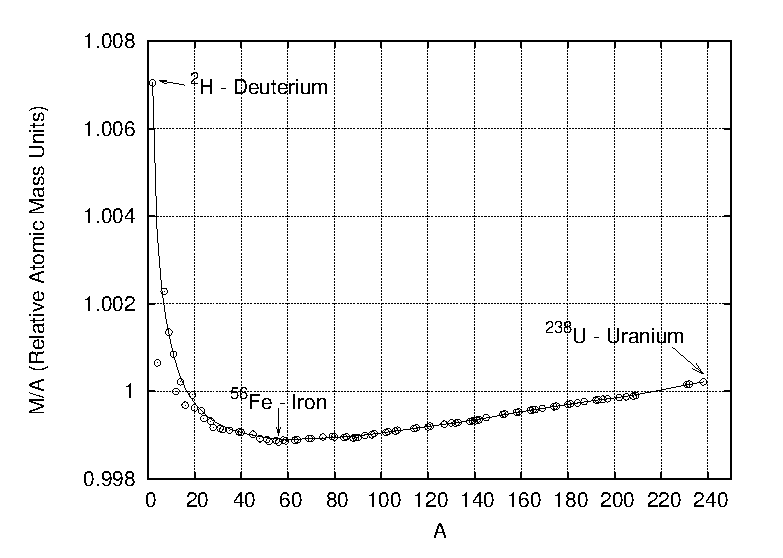
\includegraphics[width=4.5in]{relativity_conservation/mass_per_nucleon.eps}
\end{center}
\caption{Plot of mass per nucleon (proton and neutrons) for the 
elements versus the number of nucleons $A$. (Data from NIST:
http://physics.nist.gov/PhysRefData/Compositions/)}
\label{fig:mass_per_nucleon}
\end{figure}

Figure \ref{fig:mass_per_nucleon} shows a plot of the masses of the
elements, divided by the total number of protons and neutrons
(nucleons) in the nucleus of each atom.  This plot is very
illuminating when considering fusion and fission processes.  
The
fusion of two $^2$H nuclei to form a single $^4$He nucleus results in
a lower overall mass, since the number of nucleons does not change; 
consequently, this process releases kinetic
energy.  On the other hand, elements with large atomic number $A$
have a larger mass/nucleon than those with intermediate values of $A$;
consequently, kinetic energy can also be released by splitting up one of
these heavier atoms (fission).

Of the two processes --- fission and fusion --- fission is a much
easier process to achieve in the laboratory or in industrial
processes.  Many large nuclei are naturally unstable, e.g., $^{235}$U can
spontaneously decay via the fission process ${}^{235}\text{U} \rightarrow
{}^{134}\text{Xe} + {}^{100}\text{Sr} + {}^1n$.  Practically, then, the
issue boils down to setting things up such that the process can be
accelerated when desired, and can be inhibited when unwanted.  From
that perspective, the concept of a chain reaction is relevant.  The
idea of combining multiple nuclear fissions into chain reactions ---which was pioneered
by Lise Meitner, Otto Hahn, Fritz Strassmann, and Enrico Fermi in the
1930s --- is straightforward: if the neutrons that are released in a
fission process bombard another nearby (unstable) nucleus, they can
trigger the fission of that nucleus as well.  Practically, all that is
needed is a large enough density of the unstable nucleus (e.g., $^{235}$U)
 and a chain
reaction will start.  This idea was pursued by the Manhattan Project
in the 1940s to develop an atomic bomb, the detonation of which was
achieved by explosively compressing a uranium sample to increase its
density above the critical value for a chain reaction.  Alternatively,
the strength of the fission chain reaction 
can be controlled by absorbing some of the neutrons
produced in the fission reaction. Graphite  rods
(which absorb neutrons) are commonly used to ``moderate''
the reaction in this way to allow the reaction to proceed in a
controlled manner in power generators.

Nuclear fission power has a few serious drawbacks: (a) the fuel (uranium,
plutonium, etc.) is
expensive and limited in supply.  If society were to switch entirely
to uranium-fission-based power generation, it is estimated that the supply
of uranium would last for only 50-100 years.  (b) The by-products of
the fission reaction are nuclei which themselves are unstable and
radioactive; consequently, the material poses a health hazard unless
properly stored.  (Note: some countries use  techniques to
extract additional energy from this nuclear ``waste.'')
     
Another drawback of nuclear fission reactors --- which is diminishing with
improved technology --- is the concern that they could ``melt down''
and release massive amounts of radiation (this actually happened to
the Chernobyl 4 reactor in the Soviet Union in 1986).  This threat has been
lessened recently by the development of much better systems, including
a ``melt-proof'' system with an expandable core; if the temperature of
the core exceeds a defined value, the core expands, dropping the
density of the fissile material down below its critical value and
stopping the chain reaction.  (This works even if all cooling is
stopped.)  But even this system isn't perfect, as there is always the
concern that a terrorist attack or gross human error could result in
the release of disastrous amounts of radioactive waste into the
environment.

In contrast to fission reactors,  nuclear fusion reactors use water as
their  fuel  (actually the  $^2$H  isotope  of  hydrogen, also  called
deuterium,  which is  found in  small  amounts in  water) and  produce
helium   as  a   by-product,  so   waste   disposal  is   less  of   a
problem.\footnote{Some radioactive tritium  is released in the process
  as well, but it is short-lived  with a half-life of only 12 minutes;
  consequently  there   is  no   long-term  waste  problem   with  the
  tritium. The only long-term waste would be the activated material in
  the reactor  containment vessel  itself.}  The nuclear energy  production is
also much more efficient for this  process than for fission, as can be
inferred     from     the     steepness     of    the     curve     in
Fig. \ref{fig:mass_per_nucleon}.  It is estimated that there is enough
$^2$H (deuterium) in  ocean water to power the  world's needs for many
thousands of years (if not  millions).  In fact, nuclear fusion is the
power source in  stars, including our own Sun.  It  can be argued that
almost all of the Earth's energy sources can be traced back to nuclear
fusion.
     
Nuclear fusion is not  without its problems, though.  Specifically, it
is very difficult to achieve  in a controlled manner.  Making a fusion
bomb unfortunately isn't that  difficult (relatively speaking), as a
fission  explosion can  be (and  has been)  used to  compress hydrogen
together  and cause  explosive fusion.   But to  achieve  a controlled
fusion  reaction is  a very  difficult procedure  that will  require a
significant  amount  of  ingenuity  over  the next  few  decades.   If
physicists  and engineers  manage to  overcome the  technical hurdles,
earth-based fusion reactors  could prove to be an  important source of
abundant and relatively  clean power. And in the mean  time, we can 
continue to make use of the
giant fusion reactor in space that beams energy down to earth.
% This is a
% very important technological problem --- 
% the argument can be made that
% the future of modern civilization depends on the ability of engineers
% and physicists to develop techniques to achieve cost-efficient fusion
% power generation.



\newpage

\section*{Problems}
\markright{PROBLEMS}


\begin{problem}
  A nucleus with mass $\sqrt{5}\units{GeV/$c^2$}\simeq 2.24\units{GeV/$c^2$}$ 
  in its ground state and initially at rest absorbs a photon of energy $E_1$.  
  After absorbing the photon, the nucleus is raised to an excited state, 
  with mass $5.00\units{GeV/$c^2$}$, and recoils with unknown momentum $p_3$.
  \begin{enumerate}
  \item Draw a picture of this interaction.
  \item Write down the two conservation laws in terms of $E_1$, $p_3$,
    and given numerical values.
  \item Solve for $E_1$ and $p_3$.
  \end{enumerate}
  \label{prob:rel_recoil}
\end{problem}

\begin{problem}
  Calculate the speed of the recoiling excited-state nucleus in
  problem \ref{prob:rel_recoil}.  Compare with the case of photon
  emission, done as example \ref{ex:nuclear_decay} in the text.  Are
  the recoil velocities the same for emission and absorption?
  \label{prob:rel_recoil2}
\end{problem}

\begin{problem}
  A particle of mass $m_1 = 9\units{GeV/$c^2$}$ and energy $E_1 =
  15\units{GeV}$ approaches a stationary particle of mass $m_2 =
  5\units{GeV/$c^2$}$.  The particles collide and form a single
  particle of mass $m_3$.  Determine $m_3$ by using the conservation
  laws.
\end{problem}

\begin{problem}
  An incident proton, mass $m = 938.27\units{MeV/$c^2$}$, strikes a
  target proton at rest with just enough energy to create an
  electron-positron pair.  (The two protons are still present after
  the collision.)  A positron is the antiparticle of an electron; both
  the electron and positron have masses $0.511\units{MeV/$c^2$}$.
  Calculate the minimum energy needed by the incident proton in the
  frame where the target proton is initially at rest. (Hint: After the
  collision, both protons and the electron-positron pair all move
  together with the same velocity.)
\label{prob:pair_creation}
\end{problem}

\begin{problem}
  A particle of mass $3.0\units{MeV/$c^2$}$ and momentum
  $1.0\units{MeV/$c$}$ hits and sticks to a particle of mass
  $2.0\units{MeV/$c^2$}$, initially at rest.
  \begin{enumerate}
  \item Find the mass of the composite particle and its velocity.
  \item How much kinetic energy is converted to mass?
  \end{enumerate}
\label{prob:composite}
\end{problem}

\begin{problem}
  A deuteron (mass $1875.61\units{MeV/$c^2$}$) absorbs a photon and
  splits into a proton (mass $938.27\units{MeV/$c^2$}$) and a neutron
  (mass $939.57\units{MeV/$c^2$}$).  What is the minimum energy of the
  photon required to do this?
  \label{prob:deuteron}
\end{problem}

\newpage
\begin{problem}
% 2010 version -- some problems in here.  Temporarily at least, I'm
% switching back to the 2009 version unless someone fixes this version.
%  In a fusion process, two deuterium nuclei (a proton and neutron
%  bound together), each of mass $1876.12\units{MeV/$c^2$}$, interact
%  and form two new particles: a single $^3$He (two protons and a
%  neutron) with a mass of $2809.41\units{MeV/$c^2$}$ and a free
%  neutron with a mass of $939.57\units{MeV/$c^2$}$.
%
% This is the 2009 version
%  In a fusion process, two deuterium nuclei (a proton and neutron
%  bound together) each of mass $1875.61\units{MeV/$c^2$}$ combine to
%  form a single helium nucleus of mass $3727.38\units{MeV/$c^2$}$.
%
%  \begin{enumerate}
%  \item Is rest energy converted to kinetic energy or vice-versa?
%    Support your answer.
%  \item Calculate the amount of energy that is converted.
%   \end{enumerate}
The easiest and most immediately promising nuclear reaction to be used for
fusion power is the fusion of a deuterium ($^2$H) nucleus, with mass 
$1875.61\units{MeV/$c^2$}$, and a tritium ($^3$H) nucleus, with mass 
$2808.92\units{MeV/$c^2$}$.  The fusion reaction produces a $^4$He
nucleus of mass $3727.38\units{MeV/$c^2$}$,  and a free neutron of 
mass $939.57\units{MeV/$c^2$}$:
\[ {^2_1\mbox{H}} + {^3_1\mbox{H}} \rightarrow  {^4_2\mbox{He}} + n.\]
\begin{enumerate}
\item Is rest energy converted to kinetic energy or vice-versa?
Support your answer.
\item Calculate the amount of energy that is converted.
\end{enumerate}
\label{prob:fusion}
\end{problem}



\begin{problem}
  In a fission process, a slow neutron causes a uranium nucleus
  ($\text{mass} = 218,943.42\units{MeV/$c^2$}$) to split into a barium
  nucleus (mass $=$\break $131,261.73\units{MeV/$c^2$}$) and a krypton
  nucleus ($\text{mass} = 85,629.32\units{MeV/$c^2$}$), plus two
  excess neutrons (actually 3 including the original neutron, but that
  is present before the process as well), each of mass
  $939.57\units{MeV/$c^2$}$.  Calculate the energy converted from mass
  to kinetic energy in this process.
\end{problem}



\begin{problem}
  A photon of momentum $2.0\units{MeV/$c$}$ traveling along the
  positive $x$-axis strikes a particle of mass $4.0\units{MeV/$c^2$}$,
  which is initially at rest.  The result of the collision is simply
  two photons: photon $\gamma_1$ travels backward, along the negative
  $x$-axis and photon $\gamma_2$ travels forward, along the positive
  $x$-axis.
  \begin{enumerate}
  \item Draw before and after pictures of the interaction.
  \item Find the energies of $\gamma_1$ and $\gamma_2$ after the
    collision.
  \end{enumerate}
\end{problem}

\begin{problem}
  Based on the plot in Fig.~\ref{fig:mass_per_nucleon}, answer the
  following questions:
  \begin{enumerate}
  \item Why is a fusion reaction a more efficient power source
    (``pound for pound'') than a fission reaction?
  \item A supermassive star goes supernova after it has run out of
    hydrogen to fuse, at which point it starts fusing helium into
    heavier elements, then fusing those into heavier elements, etc.,
    until it gets to iron (Fe).  Up until this point, the fusion
    reactions produce kinetic energy and heat, maintaining the star.
    But after the star has fused its materials into iron, it stops
    producing kinetic energy, collapses very suddenly and goes
    ``Blammo!!''  (This is a supernova.)  What is so special about
    iron, and why can't the star produce additional kinetic energy
    after this point?
  \end{enumerate}
\end{problem}

\newpage
\begin{problem}
  A flower absorbs a (higher energy) photon of ultraviolet light and
  emits a (lower energy) red photon. Describe what happens to the mass 
  of the flower first when it absorbs the ultraviolet photon and then
  later when it emits the red photon.  Would you expect any mass
  changes during this process to be noticeable?  Explain why or why not.
\end{problem}

\begin{problem}
  It's not just nuclear reactions that involving converting mass-energy to
  kinetic energy.  Chemical reactions, such as combustion, also do this,
  although the effect on the masses is hardly noticeable.  For instance,
  when a car burns one gallon of gasoline, $132\units{MJ}$ of energy
  is released.  Consider the total mass of the reactants (i.e., all
  the molecules of the gasoline and oxygen before the reaction) versus
  the total mass of all the molecules in the chemical products after
  the reaction.  How much mass (in kg) is lost in this reaction (i.e.,
  total mass of reactants minus total mass of products)?
\end{problem}
